\documentclass[t,french,mathserif]{beamer}

\usepackage[utf8]{inputenc}

\usepackage{graphics}
\usepackage{graphicx}
\usepackage{babel}
\usepackage{color}
\usepackage{multirow}

\usetheme{default}
\usetheme{default}
\usecolortheme{ARA}
 \definecolor{col}{rgb}{0,0.5,0.1}
 \definecolor{cit}{rgb}{0.6,0.5,1}
 \definecolor{rd}{rgb}{0.8,0.1,0.1}
 \definecolor{ve}{rgb}{0,0.6,0}
 \definecolor{bleu}{rgb}{0.2,0.2,0.7}
 %\definecolor{point}{blue!60!black}

\setbeamertemplate{navigation symbols}{}
%\setbeamertemplate{footline}[frame number]

\setbeamertemplate{footline}{
	\begin{flushright}
		\insertframenumber $\quad$
	\end{flushright}
}

\newcommand{\bibd}[1]{{\hfill \scriptsize \tiny (#1)}}
\newcommand{\rb}{\textcolor{red}}
\newcommand{\gr}{\textcolor{ve}}
\newcommand{\bl}{\Large \textcolor{bleu}}

\setbeamertemplate{headline}{
	\vspace*{-3mm}
	\begin{flushleft}
		\hfill ReEnTrust F2F Meeting - Edinburgh $\qquad$
	\end{flushleft}
	\vspace*{-3.5mm}
	\vskip0pt%
	\hskip.025\paperwidth%
	\rule[0.1ex]{0.95\paperwidth}{0.05mm}
}

\title{\huge ReEnTrust Project}
\author{\Large F2F Meeting in Edinburgh}
\date{5th of June 2019}

\begin{document}

\begin{frame}[plain]
\titlepage
\end{frame}

% - What would the mediation tool look like? (Bruno and Bénédicte) + DEMO
%    - Should we have an account for each user?
%    - What should be saved? The discussion with the mediation tool?
%    - First draft with simple pre-registered answers?
%    - What algorithm should be used?
%    - If we use a trained engine, should we show the data that is used to train it?
%    - How do we know that the trust has been rebuilt?

\begin{frame}{Mediation tool: negotiation part}
    \vspace*{8mm}
    \begin{figure}
        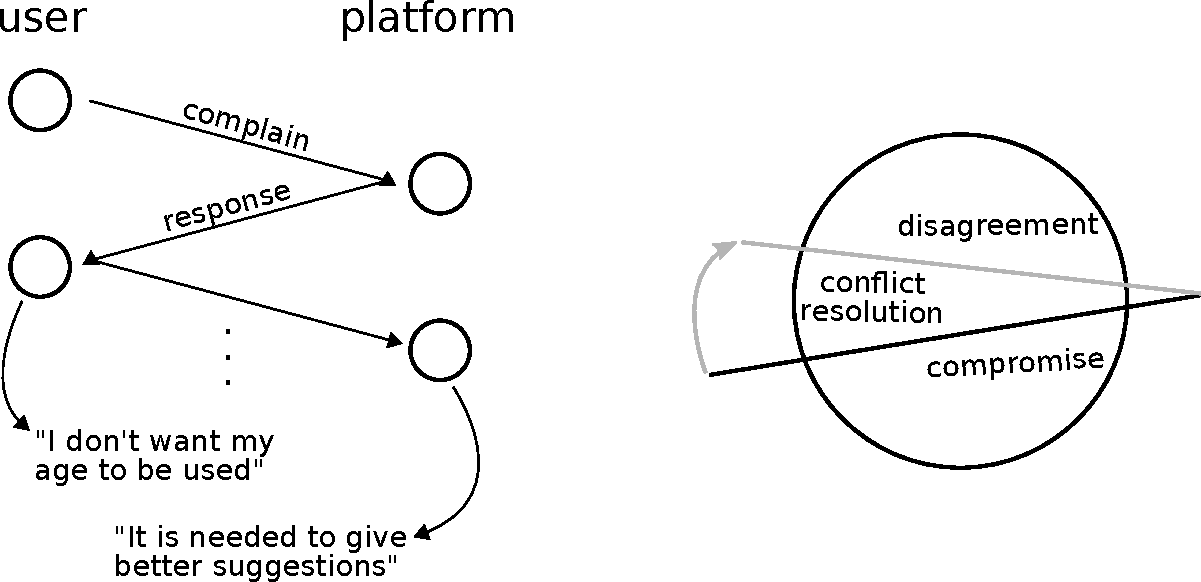
\includegraphics[scale=0.4]{negotiation.pdf}
    \end{figure}
\end{frame}

\begin{frame}{Mediation tool: negotiation part}
    \begin{itemize}
        \item User should provide:
        \begin{itemize}
            \item preferences $\rightarrow$ sandbox
            \item arguments $\rightarrow$ pre-registered
        \end{itemize}
        \item[]
        \item Platform should provide:
        \begin{itemize}
            \item explanations
            \item evidences
        \end{itemize}
    \end{itemize}
\end{frame}

\begin{frame}{Rebuilding trust}
	\begin{itemize}
        \item Refutation of users preferences and arguments must be justified
        \item[]
        \item Explaining the algorithm
        \begin{itemize}
            \item from user's claims
            \item with formal methods
            \item depending on the recommendation system
        \end{itemize}
        \item[]
        \item Showing impact of parameters and filters on:
        \begin{itemize}
            \item suggestions
            \item trust
        \end{itemize}
	\end{itemize}
\end{frame}

\begin{frame}{Compute the compromise}
	\begin{itemize}
        \item Using of formal models of negotiation protocols
        \begin{itemize}
            \item describing the conflict
            \item understanding preferences and strategies
        \end{itemize}
        \item[]
        \item Satisfy user and platform requirements?
        \begin{itemize}
            \item first step: make predictions/suggestions of responses
	        \begin{itemize}
                \item base of a dialogue between parties
                \item resulting in a balanced solution maximising their benefits
        	\end{itemize}
            \item second step: automated mediator for solutions computing
        	\begin{itemize}
                \item extracts preferences from arguments
                \item analyses the underlying game
        	\end{itemize}
        \end{itemize}
	\end{itemize}
\end{frame}

\begin{frame}{Technical questions}
	\begin{itemize}
        \item Should we have an account for each user?
        \item Should we save the conversation?
        \item What do the arguments look like?
        \item Which algorithm should be used?
        \item If we use a trained engine, should we show the data that is used to train it?
        \item How do we know that the trust has been rebuilt?
	\end{itemize}
\end{frame}

\end{document}
